\documentclass[11pt,preprint, authoryear]{elsarticle}

\usepackage{lmodern}
%%%% My spacing
\usepackage{setspace}
\setstretch{1.2}
\DeclareMathSizes{12}{14}{10}{10}

% Wrap around which gives all figures included the [H] command, or places it "here". This can be tedious to code in Rmarkdown.
\usepackage{float}
\let\origfigure\figure
\let\endorigfigure\endfigure
\renewenvironment{figure}[1][2] {
    \expandafter\origfigure\expandafter[H]
} {
    \endorigfigure
}

\let\origtable\table
\let\endorigtable\endtable
\renewenvironment{table}[1][2] {
    \expandafter\origtable\expandafter[H]
} {
    \endorigtable
}


\usepackage{ifxetex,ifluatex}
\usepackage{fixltx2e} % provides \textsubscript
\ifnum 0\ifxetex 1\fi\ifluatex 1\fi=0 % if pdftex
  \usepackage[T1]{fontenc}
  \usepackage[utf8]{inputenc}
\else % if luatex or xelatex
  \ifxetex
    \usepackage{mathspec}
    \usepackage{xltxtra,xunicode}
  \else
    \usepackage{fontspec}
  \fi
  \defaultfontfeatures{Mapping=tex-text,Scale=MatchLowercase}
  \newcommand{\euro}{€}
\fi

\usepackage{amssymb, amsmath, amsthm, amsfonts}

\def\bibsection{\section*{References}} %%% Make "References" appear before bibliography


\usepackage[round]{natbib}

\usepackage{longtable}
\usepackage[margin=2.3cm,bottom=2cm,top=2.5cm, includefoot]{geometry}
\usepackage{fancyhdr}
\usepackage[bottom, hang, flushmargin]{footmisc}
\usepackage{graphicx}
\numberwithin{equation}{section}
\numberwithin{figure}{section}
\numberwithin{table}{section}
\setlength{\parindent}{0cm}
\setlength{\parskip}{1.3ex plus 0.5ex minus 0.3ex}
\usepackage{textcomp}
\renewcommand{\headrulewidth}{0pt}

\usepackage{array}
\newcolumntype{x}[1]{>{\centering\arraybackslash\hspace{0pt}}p{#1}}

%%%%  Remove the "preprint submitted to" part. Don't worry about this either, it just looks better without it:
\makeatletter
\def\ps@pprintTitle{%
  \let\@oddhead\@empty
  \let\@evenhead\@empty
  \let\@oddfoot\@empty
  \let\@evenfoot\@oddfoot
}
\makeatother

 \def\tightlist{} % This allows for subbullets!

\usepackage{hyperref}
\hypersetup{breaklinks=true,
            bookmarks=true,
            colorlinks=true,
            citecolor=blue,
            urlcolor=blue,
            linkcolor=blue,
            pdfborder={0 0 0}}


% The following packages allow huxtable to work:
\usepackage{siunitx}
\usepackage{multirow}
\usepackage{hhline}
\usepackage{calc}
\usepackage{tabularx}
\usepackage{booktabs}
\usepackage{caption}


\newenvironment{columns}[1][]{}{}

\newenvironment{column}[1]{\begin{minipage}{#1}\ignorespaces}{%
\end{minipage}
\ifhmode\unskip\fi
\aftergroup\useignorespacesandallpars}

\def\useignorespacesandallpars#1\ignorespaces\fi{%
#1\fi\ignorespacesandallpars}

\makeatletter
\def\ignorespacesandallpars{%
  \@ifnextchar\par
    {\expandafter\ignorespacesandallpars\@gobble}%
    {}%
}
\makeatother

\newenvironment{CSLReferences}[2]{%
}

\urlstyle{same}  % don't use monospace font for urls
\setlength{\parindent}{0pt}
\setlength{\parskip}{6pt plus 2pt minus 1pt}
\setlength{\emergencystretch}{3em}  % prevent overfull lines
\setcounter{secnumdepth}{5}

%%% Use protect on footnotes to avoid problems with footnotes in titles
\let\rmarkdownfootnote\footnote%
\def\footnote{\protect\rmarkdownfootnote}
\IfFileExists{upquote.sty}{\usepackage{upquote}}{}

%%% Include extra packages specified by user

%%% Hard setting column skips for reports - this ensures greater consistency and control over the length settings in the document.
%% page layout
%% paragraphs
\setlength{\baselineskip}{12pt plus 0pt minus 0pt}
\setlength{\parskip}{12pt plus 0pt minus 0pt}
\setlength{\parindent}{0pt plus 0pt minus 0pt}
%% floats
\setlength{\floatsep}{12pt plus 0 pt minus 0pt}
\setlength{\textfloatsep}{20pt plus 0pt minus 0pt}
\setlength{\intextsep}{14pt plus 0pt minus 0pt}
\setlength{\dbltextfloatsep}{20pt plus 0pt minus 0pt}
\setlength{\dblfloatsep}{14pt plus 0pt minus 0pt}
%% maths
\setlength{\abovedisplayskip}{12pt plus 0pt minus 0pt}
\setlength{\belowdisplayskip}{12pt plus 0pt minus 0pt}
%% lists
\setlength{\topsep}{10pt plus 0pt minus 0pt}
\setlength{\partopsep}{3pt plus 0pt minus 0pt}
\setlength{\itemsep}{5pt plus 0pt minus 0pt}
\setlength{\labelsep}{8mm plus 0mm minus 0mm}
\setlength{\parsep}{\the\parskip}
\setlength{\listparindent}{\the\parindent}
%% verbatim
\setlength{\fboxsep}{5pt plus 0pt minus 0pt}



\begin{document}



\begin{frontmatter}  %

\title{Question 5: Volatility and GARCH estimates}

% Set to FALSE if wanting to remove title (for submission)




\author[Add1]{Austin Byrne}
\ead{22582053@sun.ac.za}





\address[Add1]{Stellenbosch University, Western Cape}


\begin{abstract}
\small{
This question is broken down into two sections, In section 1, I evaluate
the statement that the rand has been one of the most volatile currencies
in recent years. Tackling this question I calculate the standard
deviation of nine currencies and compare. From the plots it is evident
that the Rand is one of the most volatile in recent years. In the second
section I attampt to tackle the problem using a GARCH model.
}
\end{abstract}

\vspace{1cm}





\vspace{0.5cm}

\end{frontmatter}

\setcounter{footnote}{0}



%________________________
% Header and Footers
%%%%%%%%%%%%%%%%%%%%%%%%%%%%%%%%%
\pagestyle{fancy}
\chead{}
\rhead{}
\lfoot{}
\rfoot{}
\lhead{}
%\rfoot{\footnotesize Page \thepage } % "e.g. Page 2"
\cfoot{}

%\setlength\headheight{30pt}
%%%%%%%%%%%%%%%%%%%%%%%%%%%%%%%%%
%________________________

\headsep 35pt % So that header does not go over title




\hypertarget{introduction}{%
\section{\texorpdfstring{Introduction
\label{Introduction}}{Introduction }}\label{introduction}}

In the first part of the question I analyze the statement that the Rand
has been one of the most volatile stocks in recent years. For my
analysis I find eight other currencies of which I can compare the
volatility of the Rand to. The choice of which currencies to compare is
base on historical performance. I first analyse the standard deviation
of the currencies from prior 1990 to 2021. Over this long period it is
not evident that the rand is one of the mos volatile. More specifically
the questions states over recent years. Thus fr the next part of the
analysis I shorten the time horizon to three years, comparing the
volatility of the currencies in question to that of the Rand from 2018
to 2021. Here it is more evident that the Rand is one of the most
volatile currencies. However, the Rand is not drastically more volatile
than the Singapore, Brazilian and Indian currencies.

In the next section I dive into a GARCH model analysis. Unfortunetly I
ran out of time to do this part of the question

\hypertarget{loading-relvant-data-from-the-question}{%
\subsection{Loading relvant data from the
question}\label{loading-relvant-data-from-the-question}}

\hypertarget{evaluating-the-volatility-of-the-rand-against-other-currencies}{%
\subsection{Evaluating the volatility of the Rand against other
currencies}\label{evaluating-the-volatility-of-the-rand-against-other-currencies}}

In the first part of this question I need to comment on the statement
that the Rand has been one of the most volatile currencies. To start
this analysis I will first prepare the data available.

\hypertarget{data-preperation}{%
\subsubsection{Data preperation}\label{data-preperation}}

For this section of the analysis I will be using the cncy data set which
contains information on the currency values of 41 currencies. For the
analysis it will an over whelming amount of information if I compare the
ZAR to all of these currencies. I will therefore pick a few to do the
comparison on. The way in which I will choose which currencies to
compare the rand to is based of prior knowledge. I want to compare the
rand to the historically most volatile currencies as well as the
historically least volatile currencies and currencies that are
historically moderately volatile.

For the historically most volatile currencies I will be evaluating the
Argentinian currency, the Turkish currency and the Brazilian currency.
For the historically least volatile currencies I will be evaluating
Singapore currency, the Canadian currency and the Australian currency.
For the historically moderate currencies I will be evaluating Mexico and
India.

\hypertarget{volatility-comparison-plot-from-prior-1993-for-9-countries}{%
\subsection{Volatility comparison plot from prior 1993 for 9
countries}\label{volatility-comparison-plot-from-prior-1993-for-9-countries}}

From the plot below it is not plainly evident that the South African
currency is the most volatile. We are however, looking at a very large
scale and the question pertains to recent years. Therefore to gain a
better understanding of the volatility of the South African rand in
recent years I will look at the last 3 years of standard deviation for
each currency in question.

\begin{figure}[H]

{\centering 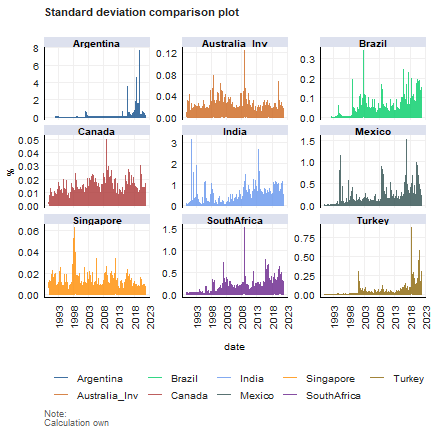
\includegraphics{Question-5_files/figure-latex/Figure 1-1} 

}

\caption{Long term volatility comparison plot \label{Figure1}}\label{fig:Figure 1}
\end{figure}

\hypertarget{volatility-comparison-plot-over-last-3-years-for-9-countries}{%
\subsection{Volatility comparison plot over last 3 years for 9
countries}\label{volatility-comparison-plot-over-last-3-years-for-9-countries}}

To gain a better understanding of the volatility of the Rand relative to
its peers in the last few years I will be shorten the time horison
inspected. The data ends in 2021. I will therefore look at the last 3
years of standard deviation. More specifically, from 2018.

From the more recent volatility plot comparison, the Rand does seem to
be one of the more volatile currencies in our data set. However, it is
not strikingly more volatile than Singapore, India or Brazil. Thus, to
conclude, the Rand has been on eo fhte more volatile currencies in
recent years.

\begin{figure}[H]

{\centering 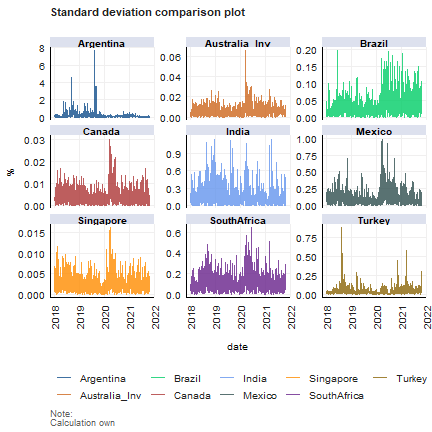
\includegraphics{Question-5_files/figure-latex/Figure 2-1} 

}

\caption{3 year volatility comparison plot \label{Figure2}}\label{fig:Figure 2}
\end{figure}

\hypertarget{references}{%
\section*{References}\label{references}}
\addcontentsline{toc}{section}{References}

\hypertarget{refs}{}
\begin{CSLReferences}{0}{0}
\end{CSLReferences}

\hypertarget{appendix}{%
\section*{Appendix}\label{appendix}}
\addcontentsline{toc}{section}{Appendix}

\hypertarget{appendix-a}{%
\subsection*{Appendix A}\label{appendix-a}}
\addcontentsline{toc}{subsection}{Appendix A}

Some appendix information here

\hypertarget{appendix-b}{%
\subsection*{Appendix B}\label{appendix-b}}
\addcontentsline{toc}{subsection}{Appendix B}

\bibliography{Tex/ref}





\end{document}
